\documentclass{scrreprt}

\usepackage{aligned-overset}
\usepackage{amsmath}
\usepackage{amssymb}
\usepackage{bm}
\usepackage[shortlabels]{enumitem}
\usepackage{hyperref}
\usepackage[utf8]{inputenc}
\usepackage{mathtools}
\usepackage{physics}
\usepackage{tabularx}
\usepackage{titling}
\usepackage{fancyhdr}
\usepackage{xfrac}
\usepackage{pgfplots}

\pgfplotsset{compat = newest}

\author{Albina Oscherowa \\ Lukas Kamratzki \\ Karsten Lehmann}
\date{SoSe 2021}
\title{Hausaufgabe 05 \\Analysis - Weiterführende Konzepte}

\setlength{\headheight}{26pt}
\pagestyle{fancy}
\fancyhf{}
\lhead{\thetitle}
\rhead{\theauthor}
\lfoot{\thedate}
\rfoot{Seite \thepage}

\begin{document}

\section*{Hausaufgabe 1}

Wir betrachten die metrischen Räume $\qty(\mathbb{R}^2, \norm{\cdot}_2)$ und
$\qty(\mathbb{R}^2, d)$, wobei $d$ die französische Eisenbahnmetrik sei.
Untersuchen Sie, welche Stetigkeitseigenschaften die folgenden Abbildungen
besitzen. \\
\begin{enumerate}[(i)]
\item $g \colon \qty(\mathbb{R}^2, d) \to \qty(\mathbb{R}^2, \norm{\cdot}_2)$
  mit $g(x) \coloneqq x$

  \textit{Lsg.} Seien $d_1$ die französische Eisenbahnmetrik und $d_2$ die von
  der euklidischen Norm induzierte Metrik.

  \textbf{Annahme}: $g$ ist Lipschitzstetig.
  \[
    \forall x, y \in \mathbb{R}^2 \colon d_2(g(x), g(y)) \leq d_1(x, y)
  \]
  \begin{minipage}[t]{.45\textwidth}
    \textbf{Fall 1}: $tx + (1 - t)y = 0, t \in \mathbb{R}$:
    \[
      \norm{x - y}_2 \leq \norm{x - y}_2
    \]
  \end{minipage}
  \vrule
  \hfill
  \begin{minipage}[t]{.45\textwidth}
    \textbf{Fall 2}:
    \[
      \norm{x - y}_2 \leq \norm{x}_2 + \norm{y}_2
    \]
  \end{minipage} \\

  Diese Aussagen sind offensichtlich war, damit ist $g$ Lipschitzstetig,
  gleichmäßig stetig und stetig.

\item $h \colon \qty(\mathbb{R}^2, \norm{\cdot}_2) \to \qty(\mathbb{R}^2, d)$
  mit $h(x) \coloneqq x$

  \textit{Lsg.} Seien $d_1$ die von der euklidischen Norm induzierte Metrik und
  $d_2$ die französische Eisenbahnmetrik.

  \textbf{Annahme}: $h$ ist Lipschitzstetig.
  \begin{align*}
    \exists L \geq 0 \forall x, y \in \mathbb{R}^2 \colon d_2(h(x), h(y)) &\leq L d_1(x, y) \\
    \text{Angenommen $x = y = (1, 0)$} \\
    \norm{x}_2 + \norm{y}_2 &\leq L \norm{x - y}_2 \\
    1 + 1 &\leq L 0 \\
    \Rightarrow h \text{ ist nicht Lipschitzstetig.}
  \end{align*}

  \textbf{Annahme}: $h$ ist gleichmäßig stetig.
  \[
    \forall \epsilon > 0 \exists \delta > 0 \forall x, y \in \mathbb{R}^2 \colon d_1(x, y) < \delta
    \Rightarrow d_2(h(x), h(y))
  \]
  \begin{minipage}[t]{.45\textwidth}
    \textbf{Fall 1}: $tx + (1 - t)y = 0, t \in \mathbb{R}$:
    \[
      \norm{x - y}_2 < \delta \Rightarrow \norm{x - y}_2 \leq \epsilon
    \]
  \end{minipage}
  \vrule
  \hfill
  \begin{minipage}[t]{.45\textwidth}
    \textbf{Fall 2}:
    \[
      \norm{x - y}_2 < \delta \Rightarrow \norm{x}_2 + \norm{y}_2 < \epsilon
    \]
  \end{minipage} \\

  Die Annahme im Fall 1 ist offensichtlich wahr.
  Sei nun neben $x$ und $y$ auch $z = (0, 0)$ aus $\mathbb{R}^2$.
  Nach der Dreiecksungleichung ist
  $\norm{x - y}_2 \leq \norm{x - z}_2 + \norm{y - z}_2$.
  Da $\norm{x - z}_2 + \norm{y - z}_2 = \norm{x}_2 + \norm{y}_2$ ist die Annahme
  im Fall 2 für $\delta = \frac{\epsilon}{2}$ wahr, somit ist $h$ gleichmäßig
  stetig.

\end{enumerate}

\newpage
\section*{Hausaufgabe 2}

Untersuchen Sie die Funktionen $f \colon \mathbb{R}^2 \to \mathbb{R}$ definiert
durch
\[
  f(x, y) = \begin{cases}
    \frac{\sin(xy)}{x} & \text{für } x \ne 0 \\
    y & \text{für } x = 0 \\
  \end{cases}
\]
auf Stetigkeit. \\

\textit{Lsg.}
\begin{center}
  \resizebox{.8\textwidth}{!}{
    \begin{tikzpicture}[
      declare function={
        f(\x, \y) = \x != 0 ? sin(deg(\x * \y))/\x : \y;
      }
    ]
      \begin{axis}[
        xlabel = $x$,
        ylabel = $y$
      ]
        \addplot3[
          surf,
          domain=-4:4,
          samples=60,
          shader=interp,
        ] {f(x, y)};
      \end{axis}
    \end{tikzpicture}
  }
\end{center}

Seien $(\mathbb{R}^2, \norm{\cdot}_2)$ und $(\mathbb{R}, \abs{\cdot})$
metrische Räume. \textbf{Vorüberlegungen}
\[
  \lim_{x \to 0} \frac{\sin(xy)}{x} = y
\]

\textbf{Annahme}: $f$ ist Lipschtzstetig.
\begin{align*}
  \exists L \geq 0 \forall (x_1, y_1), (x_2, y_2) \in \mathbb{R}^2 \colon d_2(f(x_1, y_1), f(x_2, y_2)) &\leq L d_1((x_1, y_1), (x_2, y_2)) \\
  \abs{\frac{\sin(x_1y_1)}{x_1} - \frac{\sin(x_2y_2)}{x_2}} &\leq\sqrt{(x_1 - x_2)^2 + (y_1 - y_2)^2} \\
x_1, x_2 \to 0 \quad  \abs{y_1 - y_2} &\leq L \cdot \abs{y_1 - y_2} && \Big| :\abs{y_1 - y_2} \\
  \frac{\abs{y_1 - y_2}}{\abs{y_1 - y_2}} &\leq L \\
  1 &\leq L \\
  \Rightarrow f \text{ ist Lipschitzstetig}
\end{align*}

\newpage
\section*{Hausaufgabe 3}

Wir betrachten $\qty(\mathbb{R}^N, \norm{\cdot})$ mit einer beliebigen Norm
$\norm{\cdot}$.
Beweisen Sie folgende Aussagen: Sind $A, B \subseteq \mathbb{R}^N$ kompakte
Mengen, dann sind die Mengen
\begin{enumerate}[a)]
\item $A \times B = \qty{(x, y) \middle| x \in A, y \in B} \subseteq \mathbb{R}^{2N}$ und
\item $A + B = \qty{x + y \middle| x \in A, y \in B} \subseteq \mathbb{R}^N$
\end{enumerate}
ebenfalls kompakt. \\

\textit{Lsg.}
\begin{enumerate}[a)]
\item Seien $A, B \in \mathbb{R}^N$ beschränkte und abgeschlossene Teilmengen
  und $\qty(x_n)$ eine Folge in $A \times B$.
  Weiterhin sei $x_n = \qty(a_n, b_n)$ mit $a_n \in A$ und $b_n \in B$.

  Nach Proposition 6.4.2 der Vorlesung -
  ``Ein metrischer Raum ist genau dann kompakt, wenn er folgenkompakt ist'' -
  folgt, dass $A$ und $B$ folgenkompakt sind.
  Damit existieren konvergente Teilfolgen $a_{n_j}$ und $b_{n_j}$ mit
  $\lim_{j \to \infty} a_{n_j} = a \in A$ und $\lim_{j \to \infty} b_{n_j} = b \in A$.
  Somit ist $\lim_{j \to \infty} u_{n_j} = \qty(a, b) \in A \times B$.
  $\Rightarrow A \times B$ ist folgenkompakt.

\item Seien $A, B \in \mathbb{R}^N$ beschränkte und abgeschlossene Teilmengen.
  Dann existieren nach $(A13)$ auch $\inf A, \sup A$ und $\inf B, \sup B$.
  Die Menge $A + B$ ist durch $\sup A + \sup B$ nach oben und durch
  $\inf A + \inf B$ nach unten beschränkt.

  Jede Folge $\qty(x_n)$ aus $A + B$ lässt sich durch $x_n \coloneqq a_n + b_n$
  mit $\qty(a_n) \in A$ und $\qty(b_n) \in B$ beschreiben.
  Falls $\lim_{n \to \infty} x_n = x$ existiert, dann ist
  $x = \lim_{n \to \infty} a_n + \lim_{n \to \infty} b_n$.
  Da $A$ und $B$ abgeschlossen sind liegt $a \in A$, $b \in B$
  und $x \in A + B$.
  Damit ist $A + B$ ebenfalls abgeschlossen und kompakt.
\end{enumerate}

\end{document}
